\documentclass[12pt, a4]{article}
\usepackage[T1]{fontenc}
\usepackage{graphicx}
\usepackage[brazil]{babel}
\usepackage{mathtools}
\usepackage{amsmath,array}
\usepackage{longtable}
\usepackage{enumitem}
\usepackage{float}
\usepackage{tikz}

\begin{document}
\begin{titlepage}

\newcommand{\disciplina}{Processamento de Materiais I: Solidificação e Fundição (SMM 0302)}
\newcommand{\titulo}{Desafio PBL Tupy x USP 2025: Primeira Entrega}


\newcommand{\prof}{Prof. Dr. Marcelo Falcão de Oliveira}
\newcommand{\data}{São Carlos,\\ 12 de setembro 2025}



\center


\begin{tikzpicture}[remember picture,overlay]
   
    \node[anchor=north west, xshift=1cm, yshift=-1cm] at (current page.north west) 
    {
\includegraphics[scale=0.6]{eesclogo.png}};
    
    \node[anchor=north east, xshift=-1cm, yshift=-1cm] at (current page.north east) 
    {
\includegraphics[scale=0.6]{tupylogo.png}};
\end{tikzpicture}


\textbf{\Large\titulo}

\begin{center}
    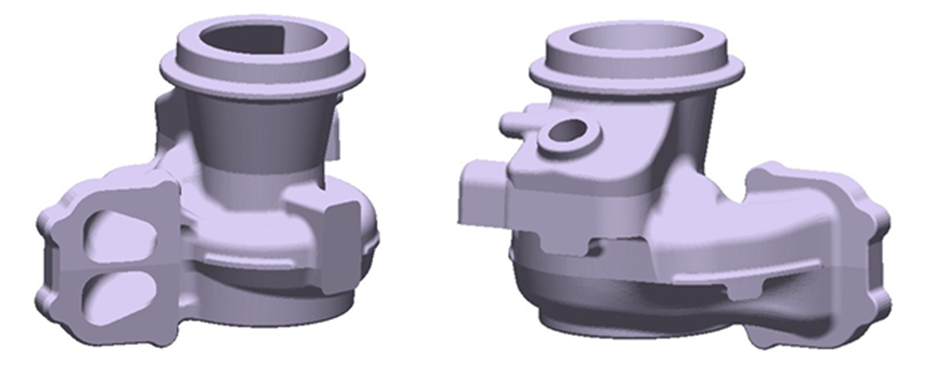
\includegraphics[scale=0.8]{peca1.png}
\end{center}



\textbf{\disciplina}

\vspace{0.5cm}

\textbf{\prof}

\vspace{0.5cm}

\begin{flushright}
\begin{tabular}{l l}
    Ana Julia Borges Guerra & 11799962\\
    Guilherme Capputti Mazzini & 14099960\\
    Ítalo Cunha Melo Silva & 11223292\\
    Murilo Fernandes Pinto & 14599895\\
    Ricardo Rodrigues da Silva & 14616503
\end{tabular}
\end{flushright}

\vfill
\data

\end{titlepage}
\pagebreak

\begin{flushleft}
    \textbf{Objetivos}
\end{flushleft}

O objetivo deste projeto é o desenvolvimento de um molde para a produção conjunta de duas carcaças de turbina em ferro fundido nodular, visando identificar e reproduzir as dificuldades encontradas no processo industrial. Nesta primeira entrega, busca-se elaborar o conceito do molde em 3D por meio de softwares de CAD e também com auxílio do Inspire Cast, acompanhado das justificativas e das estratégias adotadas quanto aos componentes do sistema e posicionamentos. As etapas seguintes do projeto irão contemplar a realização de simulações para validar o desempenho do sistema proposto, garantindo o cumprimento dos requisitos da empresa: peça isenta de defeitos nas regiões críticas apresentadas no PDF fornecido pela Tupy, vazamento a 1420 °C e temperatura mínima de 1250 °C ao final do enchimento, uso de dois corpos de prova por molde com dimensões predefinidas e rendimento metalúrgico mínimo de 50\%.

\begin{flushleft}
    \textbf{Introdução}
\end{flushleft}

O presente relatório apresenta as estratégias iniciais para solucionar o desafio proposto pela empresa Tupy S.A para o ano de 2025. Nesse desafio, busca-se projetar um molde com os diversos elementos possibilitadores do processo de fundição e solidificação de duas carcaças de turbina. Para verificação do modelo proposto pelo grupo, nas próximas etapas e entregas do projeto serão feitas simulações no software Inspire Cast da Altair. 

A grande importância do trabalho reside no fato de que processos de fundição são complexos: envolvem um bom planejamento aplicando conhecimentos em transporte de matéria, transferência de calor, ciência e engenharia de materiais. Um produto fundido que não teve seu processamento adequadamente planejado pode apresentar problemas funcionais e de qualidade, trazendo desperdícios e prejuízos financeiros.

 Inicialmente, é feita uma simulação apenas com a peça (sem nenhum elemento do sistema de alimentação ou de enchimento). É esse o passo inicial para que seja possível identificar as regiões que solidificam por último e as porosidades: isso guiará o grupo à definição de posicionamento de massalotes e luvas. É uma etapa fundamental para evitar rechupes e problemas de contração. Nas futuras simulações, será testado todo o molde em conjunto com a peça e questões mais complexas serão analisadas: dimensionamento dos massalotes, velocidade do fluxo devido aos canais de vazamento escolhidos, entre outros. 


\begin{flushleft}
    \textbf{Massalotes e Resfriadores}
\end{flushleft}

O correto posicionamento de resfriadores e massalotes é indispensável para eliminar as porosidades causadas pela contração da liga durante a solidificação. As contrações na peça, supondo o sucesso dos canais de alimentação em distribuir o metal de forma homogênea, ocorrem nas últimas regiões a se solidificarem, geralmente nas áreas de maior espessura da peça, que correspondem a volumes maiores do molde. Em peças com geometrias mais complexas, como no caso deste projeto, as porosidades de contração (rechupe) surgem em diversas regiões de elevada espessura local, em vez de se concentrarem em uma única região — normalmente no centro da peça, como ocorre em geometrias simples. Nesse contexto, os componentes do sistema devem atuar de forma complementar para garantir o sucesso da solidificação direcional.
Uma análise prévia da solidificação da peça deste projeto mostrou uma concentração significativa de porosidades no equador da peça e na parte superior (regiões destacadas no material de apresentação do desafio), justamente nas zonas de maior espessura, como previsto. A estratégia utilizada pela equipe foi empregar massalotes para garantir a alimentação de metal líquido diretamente no equador da peça e aplicar resfriadores nas regiões periféricas de ocorrência de porosidade, de modo a aumentar o fluxo de calor e favorecer a solidificação adequada nessas áreas.

\begin{figure}[!htb]
\begin{center}

    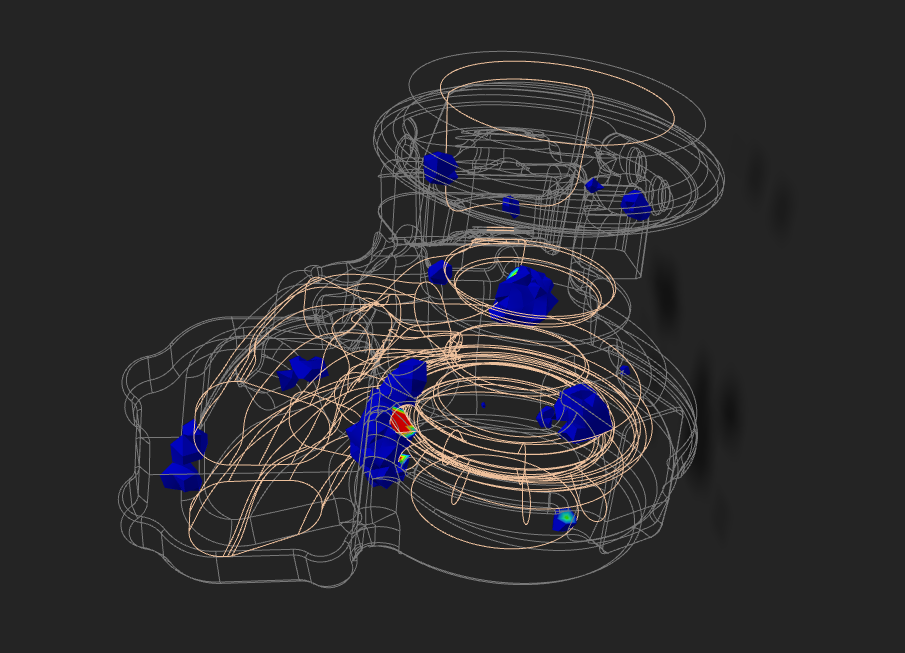
\includegraphics[scale=0.5]{simulacao1.png}
\end{center}
\end{figure}


\end{document}